\chapter{Вычисление в гетерогенных вычислительных средах}\label{ch:ch2}

\section{Проблемы распараллеливание алгоритмов класса SPH на гетерогенных вычисленных системах с разделяемой памятью}\label{sec:ch2/sec1}

В классической задаче \(N\) тел при расчете силы, действующей на любой объект, необходимо учитывать влияние на этот объект всех тел в системе, из чего следует, что для таких алгоритмов характерна квадратичная асимптотическая сложность \(O(N^2)\). Это одна из ключевых проблем любой численной модели на основе частиц, так как при существовании требования большей детализации возникает необходимость использовать большого количества частиц. В свою очередь для вычисления следующего состояния системы для каждой частицы важно знать физические параметры любой другой частицы.

Комбинированный метод PIC (PIC – particle in cell) \cite{Harlow1963, Grigoriev2000, Belocherkovsky1982} и его модификации \cite{Belocherkovsky1982}, предполагают, что сплошная среда описывается как частицами так и фиксированной сеткой. При этом частицы несут в себе информацию лишь о массе в то время как информация об флуктуациях физических величин в системе распространяется через фиксированные узлы сетки.
Таким образом для синхронизации параллельных вычислений на различных узлах кластера или устройствах одного узла достаточно лишь своевременного обновления значений в узлах сетки и информацию о количестве частиц в ячейки.

В то же время полностью Лагранжевые алгоритмы такие как SPH система координат связана с движением жидкости в пространстве (сетка движется вместе с жидкостью) и отвечает фиксированным точкам в среде. Таким образом сплошная среда представляется как дискретное множество частиц. Информация в среде передается исключительно через частицы, что делает трудным распараллеливание вычислений на разных физических узлах кластера или между GPU (графический сопроцессор) в пределах одного вычислительного узла или устройства. Для численных моделей основанных на системе частиц, не смотря на то, что каждый метод хорошо распараллеливаются по данным, представляется довольно сложным распределение вычислений на системах с не общей памятью - такие как узлы кластера общающиеся по сети или различные вычислительные устройства в рамках одной машины, но независимыми модулями оперативной памяти (GPU). Это в частности обусловлено тем,  что частицы динамичны и не привязаны к определенным позициям, как узлы расчетных сеток. Тем ни менее, в работах \cite {Dominguez2013, Verma2017, Verma2018} предложены попытки преодолеть этот недостаток за счет логичного разделения моделируемого пространства на не пересекающиеся статичные или динамичные подпространства - домены. Таким образом частицы можно кластеризовать по пространственному признаку, в зависимости от текущей позиции. При этом подразумевается, что каждый домен обрабатывается отдельным  устройством - вычислителем. В нашей интерпретации метода PCI SPH мы также основывались на этом подходе ниже в таблице \ref{tab:algocmp1} представлено сравнение между нашим и аналогичными подходами.

\begin{table} [htbp]% Пример записи таблицы с номером, но без отображаемого наименования
  \centering
  \begin{threeparttable}% выравнивание подписи по границам таблицы
    \caption{Реализации подходов распараллеливания методов частиц на нескольких устройствах}%
    \label{tab:algocmp1}%
    \begin{SingleSpace}
      \begin{tabular}{| c | c | c | c |}
        \hline
        Источник              & \thead{Технология \(||\) вычислений} & Алгоритм & \thead{Доступность (Open source) } \\ \hline
        \cite {Dominguez2013} & CUDA + MPI                           & SPH      & -                                  \\ \hline
        \cite {Verma2017}     & CUDA                                 & SPH      & -                                  \\ \hline
        \cite {Verma2018}     & CUDA                                 & PCI SPH  & -                                  \\ \hline
        Sibernetic            & OpenCL                               & PCI SPH  & +                                  \\ \hline
      \end{tabular}%
    \end{SingleSpace}
  \end{threeparttable}
\end{table}

\section{Алгоритм поиска соседей}\label{sec:ch2/sect2}
Наряду с неэффективным методом перебора всех частиц были предложены другие алгоритмы, базирующиеся на пространственном делении всей области на ячейки \cite {Teschner2003, Kipfer2006, Keiser2006, Cohen1995}. Подобные алгоритмы предполагают, что можно пренебречь незначительным влиянием частиц, находящихся на расстоянии, превышающем определенную длину сглаживания  рисунок ~\ref{fig:ns_1}.
\begin{figure}[ht]
  \centerfloat{
    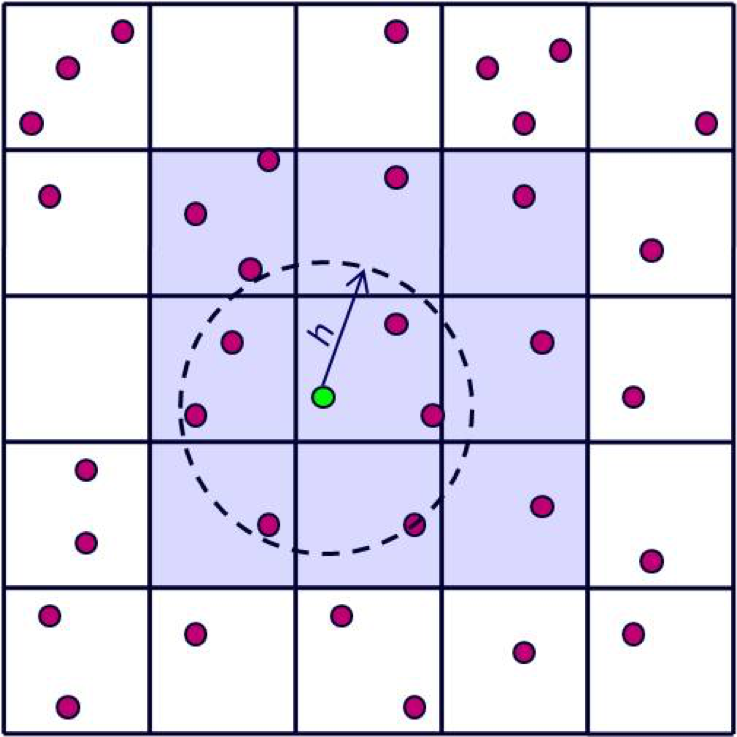
\includegraphics[scale=0.30]{ns_1}
  }
  \caption{Поиск соседей в ближайших смежных ячейках.
  }\label{fig:ns_1}
\end{figure}
Это позволяет свести сложность алгоритма к \(O(M \cdot N)\), где \(M < N\).

Использование подобных методов позволяет в целом сократить количество вычислений, однако необходимо помнить, что, наряду с остальными задачами, возникает проблема, связанная обновлением списка соседей для каждой частицы каждую итерацию. «Поиск соседей» является одной из самых важных стадий алгоритма и одной из самых трудоемких операций. Как правило, она занимает порядка 30\% времени работы симуляции за один шаг. Существует два способа кластеризации частиц в пространстве в зависимости от их текущих позиций - KD-дерево и пространственный хеш. Основным недостатком KD-деревьев является необходимость перестраивать их на каждой итерации в связи с тем, что система динамична таблица \ref{tab:algoNS1}.

\begin{table} [htbp]% Пример записи таблицы с номером, но без отображаемого наименования
  \centering
  \begin{threeparttable}% выравнивание подписи по границам таблицы
    \caption{ Алгоритмы поиска списка соседей. }%
    \label{tab:algoNS1}%
    \begin{SingleSpace}
      \begin{tabular}{| c | c | c |}
        \hline
        Название                     & +                                     & -                                      \\ \hline
        Перебор                      & Простота реализации                   & {\makecell { Aсимптотическая сложность \\ \( O(n^2)\) }} \\ \hline
        KD-дерево                    & {\makecell {Быстро и эффективно можно                                          \\
        находить ближайших соседей}} & {\makecell {Необходимо перестраивать                                           \\ дерево на каждой итерации \\
        (система динамична)}}                                                                                         \\ \hline
        Хеш функция                  & {\makecell {Быстро и эффективно                                                \\ можно находить \\ ближайших соседей }} & {\makecell {Сортировка массива \\ частиц на \\ каждой итерации }} \\ \hline
      \end{tabular}%
    \end{SingleSpace}
  \end{threeparttable}
\end{table}

Алгоритм разбит на несколько стадий, каждая из которых описана ниже. На начальном этапе пространство делится на равные ячейки, ширина, длина и глубина которых равна \(2h\) ( \(h\)радиус сглаживания); инициализируются специальные списки, в которых будет храниться информация о соседних частицах. Для алгоритма PCI SPH верно следующее утверждение: количество частиц в любом объеме ограничено константой. В силу того, что алгоритм PCI SPH моделирует несжимаемую жидкость можно утверждать, что количество частиц в в любом объеме не должно  превосходить некоторое число, что бы поддерживалось условие не сжимаемости. То есть плотность моделируемой не должно превосходить стандартную плотность более чем на заданный процент. Отсюда можно оценить максимальное количество частиц в каждой пространственной ячейки исходя из пространственных параметров ячейки. По нашим оценкам, для реализации алгоритма PCI SPH \(M\) не превосходит 1220 в силу не сжимаемости жидкости.

На втором этапе для каждой частицы, вычисляется пространственный индекс ячейки, в которой она находится в текущий момент времени \cite {Teschner2003} полученный индекс помещается в массив \(particleIndex\).  Индекс зависит от позиции частицы и вычисляется следующим образом:
\[
  cell(x,y,z,h) = \left( \left \lfloor \frac{x - x_{min}}{2h} \right \rfloor, \left \lfloor \frac{y - y_{min}}{2h} \right \rfloor, \left \lfloor \frac{z - z_{min}}{2h} \right \rfloor \right ) = (i,j,k)
\]
\[
  cellID = j + k \cdot gridCellY + i \cdot gridCellZ \cdot gridCellY
\]

Заполненный массив \(particleIndex\) сортируется по ячейкам алгоритмом быстрой сортировки рисунок ~\ref{fig:ns_2}, в соответствии с этим списком сортируются позиции и скорости, соответствующие значения помещаются в специальные временные списки.
\begin{figure}[ht]
  \centerfloat{
    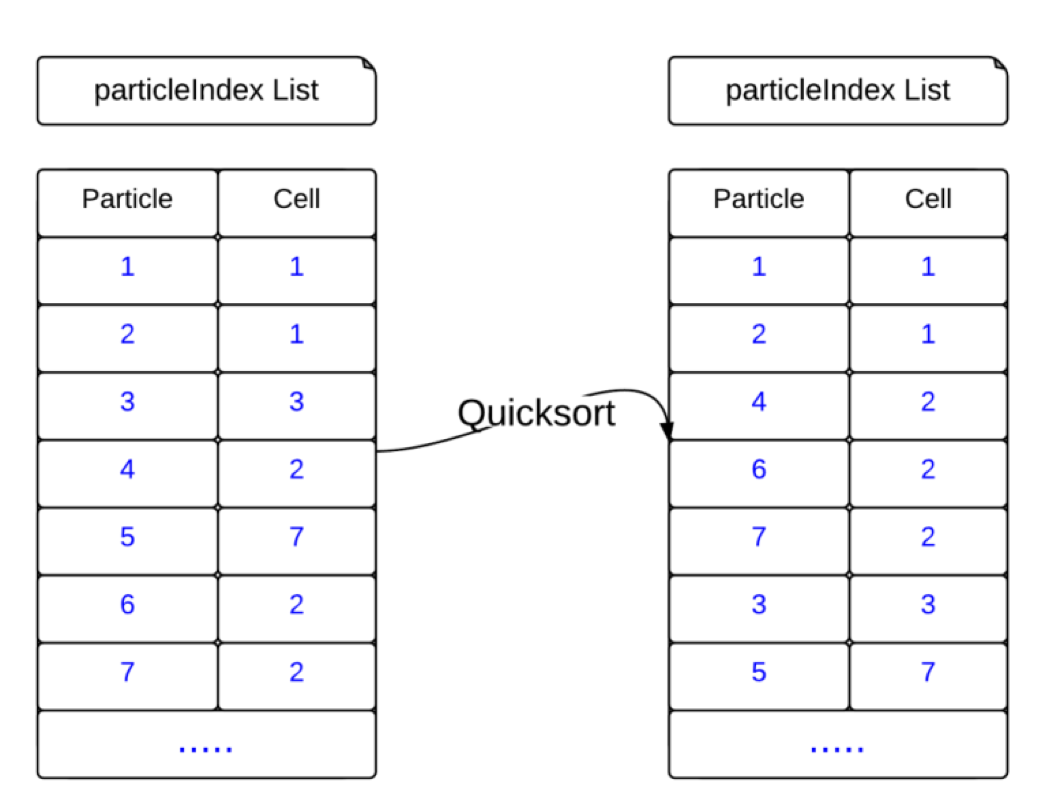
\includegraphics[scale=0.30]{ns_2}
  }
  \caption{Список \(particleIndex\) после сортировки.}
  \label{fig:ns_2}
\end{figure}

Все это позволяет быстро извлекать значения скоростей и позиции частиц, лежащих в определенной ячейке. Однако после сортировки позиции в списке \(particleIndex\) не соответствуют списку позиций частиц, и довольно проблематично отслеживать изменения свойств одной определенной частицы. Для решения этой проблемы был введен список \(particleIndexBack\), который дублирует список \(particleIndex\) до сортировки рисунок ~\ref{fig:ns_3}, это позволяет, в том числе, эффективно отлаживать приложение в условиях параллельного программирования.
\begin{figure}[ht]
  \centerfloat{
    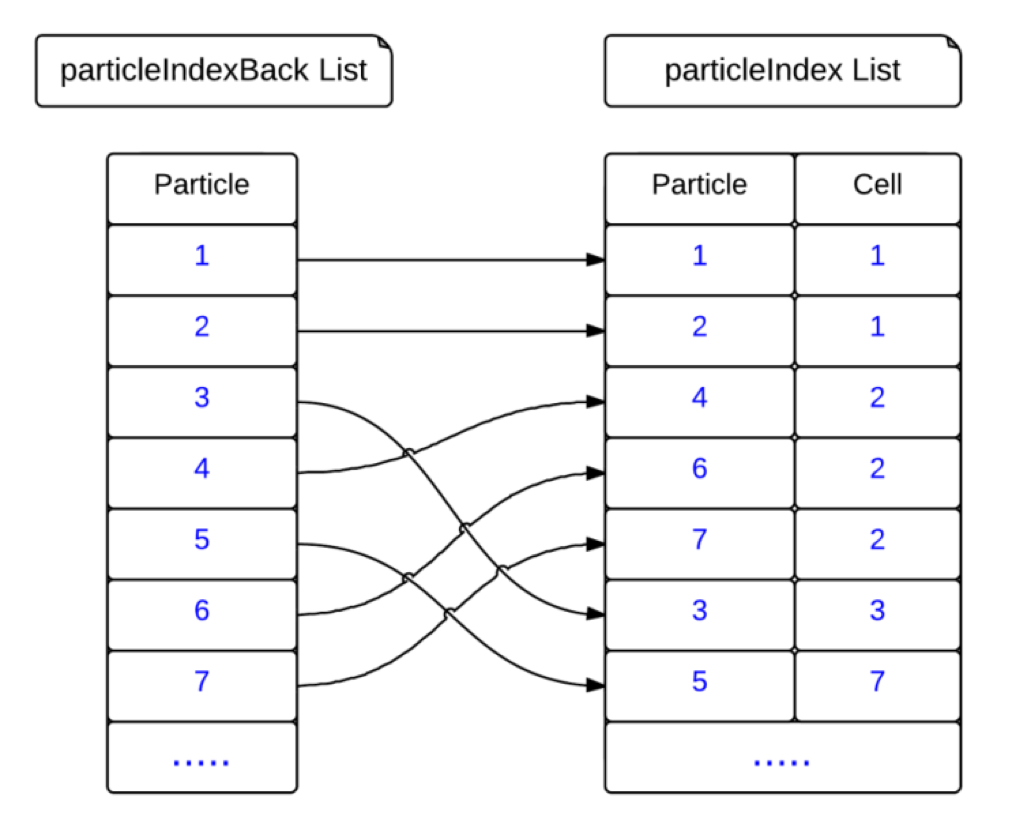
\includegraphics[scale=0.30]{ns_3}
  }
  \caption{Связь между списком \(particleIndexBack\) и \(particleIndex\).}
  \label{fig:ns_3}
\end{figure}

На третьей стадии алгоритма, при непосредственном поиске соседей, для каждой частицы среди потенциальных соседних частиц (частиц которые находятся не дальше чем \(h\)) необходимо отобрать не более 32 ближайших. Поиск потенциальных соседей в первую очередь проходит в «домашней» ячейке (ячейка, в которой на данный момент находится частица), затем вычисляется положение частицы в ячейке, для этого ячейка разбивается на 8 равных пространственных фрагментов с длиной грани равной радиусу сглаживания рисунок ~\ref{fig:ns_4}.
\begin{figure}[ht]
  \centerfloat{
    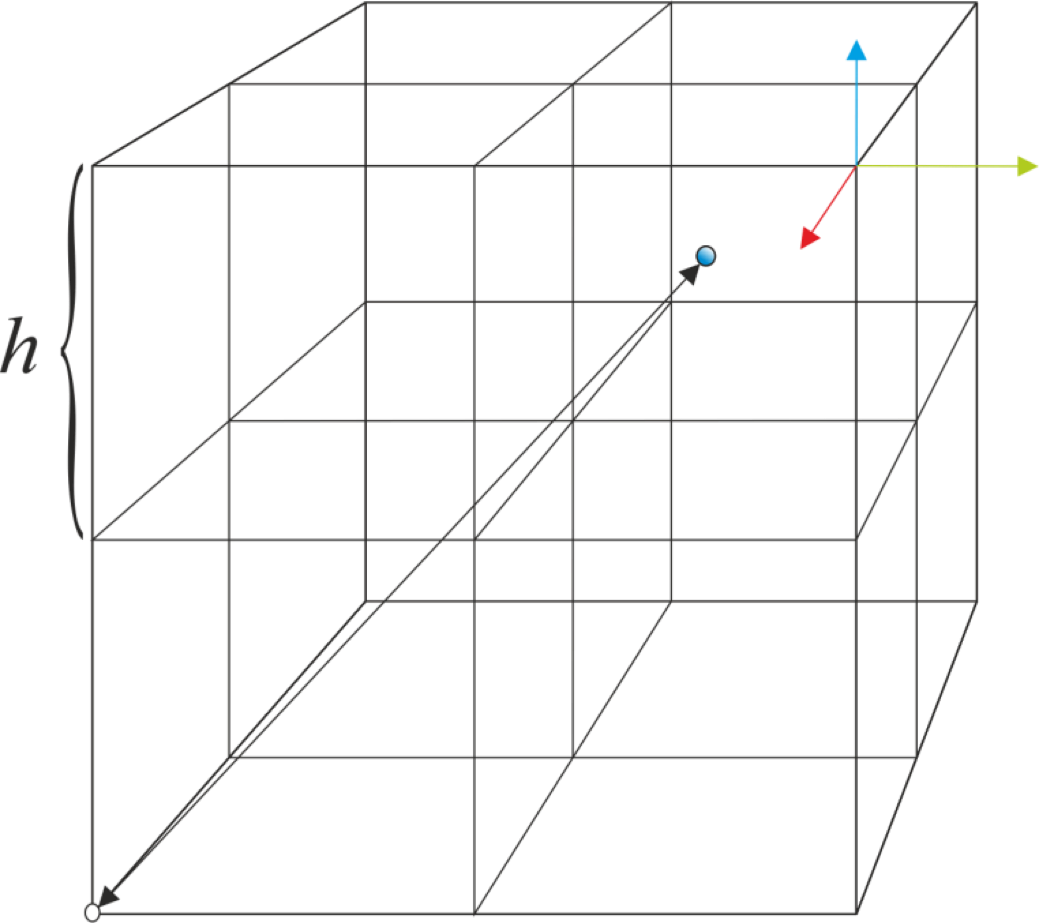
\includegraphics[scale=0.20]{ns_4}
  }
  \caption{Разбиение ячейки на 8 равных фрагментов.}
  \label{fig:ns_4}
\end{figure}

Поиск оставшихся «потенциальных» соседей проходит в семи смежных для пространственного фрагмента ячейках. Это позволяет избежать вычислений, связанных с рассмотрением частиц, лежащих заведомо дальше, чем радиус сглаживания.

Формально можно представить список соседей как множество индексов частиц \(N_{i,h}=\left \{ j|\left | r_i-r_j \right | \leqslant h \right \}\). Для того чтобы отобрать наиболее близкие частицы, сначала необходимо выяснить на каком минимальном расстоянии \(h_min \leq  h\) находится удовлетворяющее нас количество ближайших частиц \(N_{i,h_{min}}=\left \{ j|\left | r_i-r_j \right | \leqslant h \right\} \subseteq N_{i,h}\). Для этого анализируется множество \(Nd_i=\left \{ k_{i,j}|k_{i,j}=\left | N_{i,\frac{h\cdot j}{s}} \right | - \left | N_{i,\frac{h\cdot (j-1)}{s}} \right |, j\in [1,...,s] \right \}\), где \(s=30\), и для частицы \(i\) получает \(h_{min}=\frac{(j+1)\cdot h}{s} |  j = \max_{1\leq c\leq s}\left ( c|\sum_{l=1}^{c} k_{i,l} \right )\leq NeighbourCount, k_{i,l} \in Nd_j\) \(NeighbourCount=32\) ~\ref{fig:ns_5}.
\begin{figure}[ht]
  \centerfloat{
    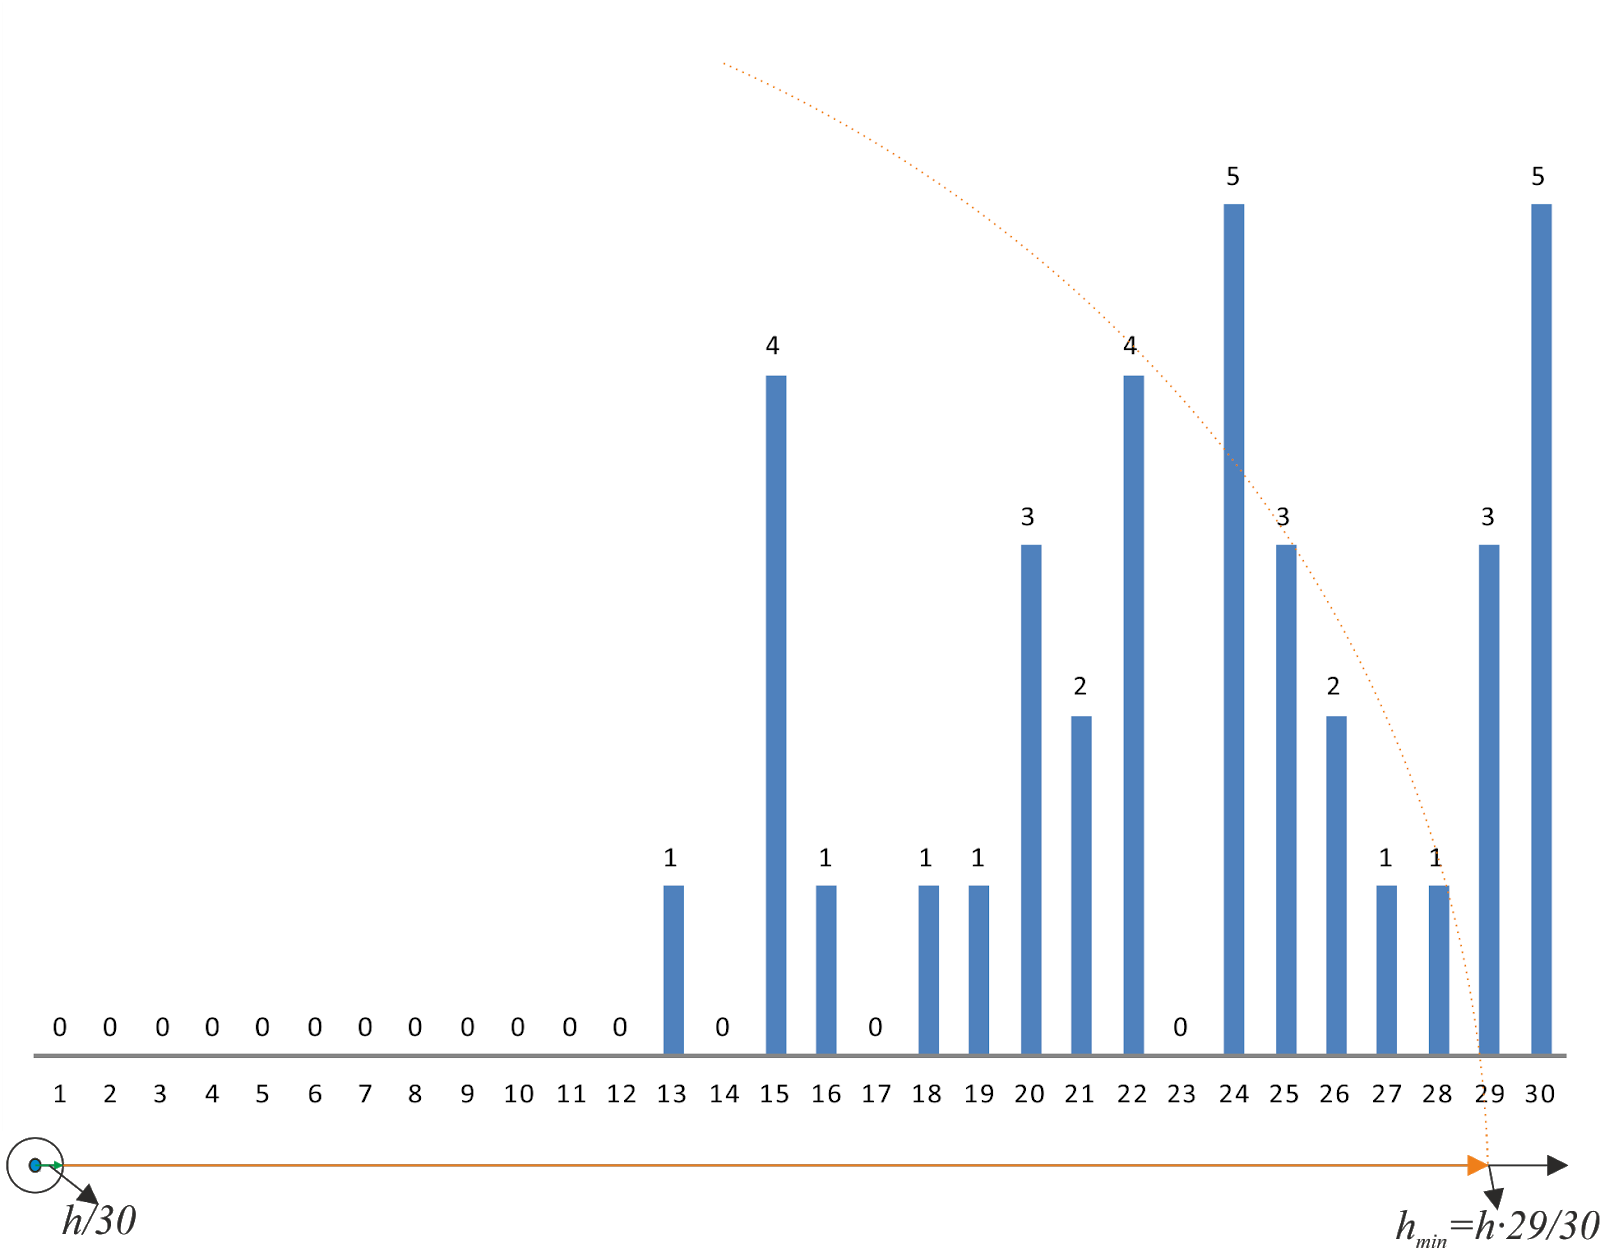
\includegraphics[scale=0.20]{ns_5}
  }
  \caption{Иллюстрация принципа выбора минимального радиуса. Гистограмма распределения расстояний от данной частицы \(i\) до соседних частиц. На данном примере достаточное количество соседних частиц, а именно 32, находится внутри сферы радиусом.}
  \label{fig:ns_5}
\end{figure}
Ниже приведена схема алгоритма поиска соседей ~\ref{algo:ns}.

\begin{algorithm}[H]
  \label{algo:ns}
  \SetAlgoLined
  \SetKwFunction{Neighbour}{Neighbour}
  \SetKwFunction{PutNeighbour}{PutNeighbour}
  \SetKwFunction{SearchParticlesForCell}{PutNeighbour}
  \SetKwFunction{Dist}{Dist}
  \SetKwInOut{Input}{input}\SetKwInOut{Output}{output}
  \Input{$\mathcal P$ множество частиц}
  \Input{$\mathcal N_{map}$ список списков всех соседей для каждой частицы}
  \Input{$\mathcal C$ список пространственных ячеек }
  \ForEach{$p \in \mathcal P$}
  {
    $r_s  \leftarrow 30 $\;
    $array[1...r_s]\, r_d \leftarrow [0...0]$\;
    $searchMode \leftarrow false$\;
    $h_{min} \leftarrow h$\;
    \textbf{search}: \\
    \ForEach{$c \in \mathcal C$}
    {
      $P_c \leftarrow \left \{ \mathcal P_c \subseteq \mathcal P| \forall p_{i}\in \mathcal P_{c} \Rightarrow p_{i}.cellID = c \right \} $\;
      \SearchParticlesForCell{$\mathcal N_{map}$[p], $h_min$, $searchMode$}\;
      $searchMode \leftarrow true$\;
      \If{$searchMode == true$}{
        $n_{c} \leftarrow 0$\;
        \ForEach{$j \in [1...r_{s}]$}{
          $n_{c} \leftarrow n_c + r_{d}[j]$\;
          \If{$n_c > 32$}{
            $h_{min} \leftarrow (j-1)\cdot \frac{h}{r_s}$ \;
            \textbf{goto search}\;
          }
        }
      }
    }
  }
  \caption{Схема алгоритма поиска соседей}
\end{algorithm}

Процедура поиска множетва частиц в пространственной ячейке \(c\) описана в схеме ~\ref{algo:ns_c}.

\begin{algorithm}[H]
  \label{algo:ns_c}
  \SetAlgoLined
  \SetKwFunction{Neighbour}{Neighbour}
  \SetKwFunction{PutNeighbour}{PutNeighbour}
  \SetKwFunction{Dist}{Dist}
  \SetKwInOut{Input}{input}\SetKwInOut{Output}{output}
  \Input{$\mathcal P_c$ множество частиц для ячейки c}
  \Input{$\mathcal N_{map}$ список списков всех соседей для каждой частицы}
  \Input{$h_{min}$ радиус}
  \Input{$ searchMode$ режим поиска/заполенния}
  $r_s  \leftarrow 30 $\;
  $h_{min} = h$\;
  \ForEach{$p_{n} \in \mathcal P_c = \left \{ \mathcal P_c \subseteq \mathcal P| \forall p_{i}\in \mathcal P_{c} \Rightarrow p_{i}.cellID = c \right \} $}
  {
    d = \Dist($p$,$p_{n}$)\;
    \If{$d \leq h_{min}$}{
      \eIf{$searchMode \neq true$} {
        $r_{j} \leftarrow \left [ d \cdot \frac{r_{s}}{h} \right ] $\;
        $r_{d}[r_{j}] \leftarrow r_{d}[r_{j}] + 1$\;
      }
      {
        $neighbour \leftarrow Neighbour(p_{i}, d)$ \;
        \PutNeighbour{$\mathcal N_{map}$[p], $neighbour$}\;
      }
    }
  }
  \caption{Схема алгоритма поиска частиц в окресности для заданной ячейке.}
\end{algorithm}

Функция \( Dist \) - расчитавает растояние между частицами как растояние Евклида.

\section{Алгоритм распределения зависимых данных по разным вычислительным устройствам}\label{sec:ch2/sec3}
Основная идея алгоритма заключается в распределении данных между вычислительными устройствами(вычислитель). Таким образом, чтобы обеспечить каждую частицу, обрабатываемую устройством, необходимым и достаточным, массивом данных, для расчета списка соседей и физических величин. При этом количество частиц, обрабатываемых одним устройством, должно зависеть от его вычислительных возможностей. Также в следствии того, что система не статична, алгоритм должен динамически перераспределять данные между устройствами, чтобы поддерживать оптимальное распределение и актуальность данных на каждом устройстве.

Для каждая частицы в каждый момент времени известен \(cellID\)– или индекс пространственной ячейки, в которой она находиться  в момент времени t. Таким образом можно кластеризовать частицы как минимум по их \(cellID\). В то же время все моделируемое пространство можно разделять на группы пространственных ячеек. При этом вследствии  того, что нашей основной целью является распараллеливание моделирования жидкости методом PCI SPH, обоснованно предположить, что необходимо и достаточно разделять пространство по плоскости коллинеарной вектору гравитации рисунок ~\ref{fig:dstr_1}.
\begin{figure}[ht]
  \centerfloat{
    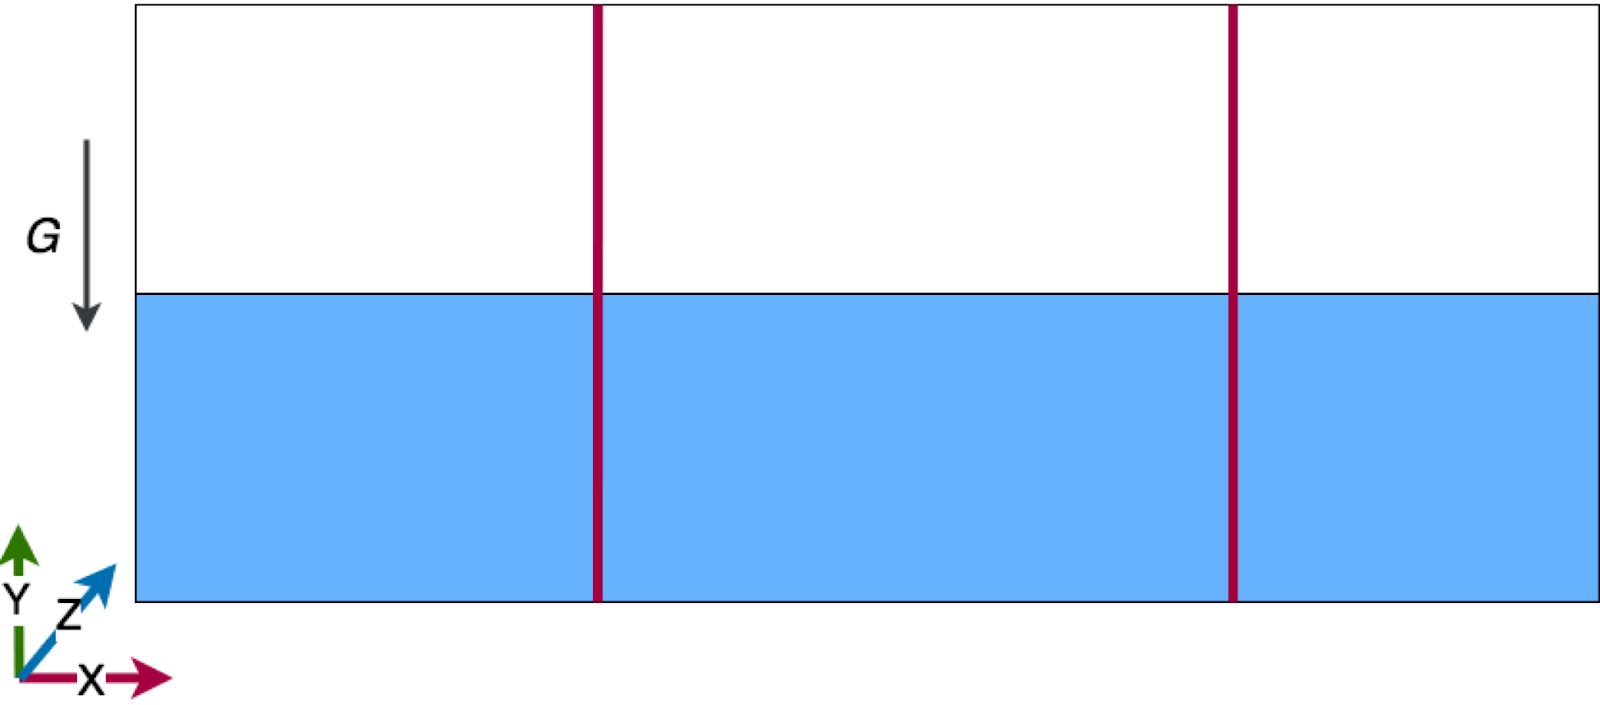
\includegraphics[scale=0.30]{distrib1}
  }
  \caption{Распределение данных между устройствами для алгоритма PCI SPH, разделение пространства показано красными вертикальными линиями, стрелкой с надписью G обозначено направление вектора гравитации.}
  \label{fig:dstr_1}
\end{figure}

Очевидно, что для обновления свойств частиц находящихся в смежных областях доменов необходимо иметь информацию о частицах находящихся в соседних ячейках из других доменов и, в тоже время, находящихся в памяти другого устройства. Для этого данные о всех частицах находящихся в таких ячейках также копируется в память вычислительного устройства, но при этом для них расчеты не производятся. Будем называть такие частицы мнимыми или неподвижными.
Синхронизация вычислений обеспечивается в двух аспектах: синхронизация времени работы - устройства выполняют свою работу одновременно, синхронизация данных - так как устройства работают с общим массивом необходимо, чтобы их работа, не влияла на целостность и структуру данных. Таким образом алгоритм должен удовлетворять следующему ряду требований:
\noindent Вложенные списки:
\begin{itemize}
  \item Масштабируемость относительно количества доступных вычислительных устройств.
  \item Устройства должны работать независимо.
  \item Устройства должны работать синхронно, т.е.:
        \begin{itemize}
          \item Устройства начинают исполнение  одновременно.
          \item Среднее время работы устройств отличается на допустимую погрешность.
        \end{itemize}
  \item Для каждого устройства программа должна автоматически определять количество обрабатываемых данных.
\end{itemize}

Входные данные для алгоритма состоят из начальных отсортированного по  \(cellID\) массива частиц; а также и из данных об устройствах – количество, весовые коэффициенты распределения данным между устройствами вычисляются автоматически. На рисунке \ref{fig:dstr_2} показан пример разбиения данных на партиции
\begin{figure}[ht]
  \centerfloat{
    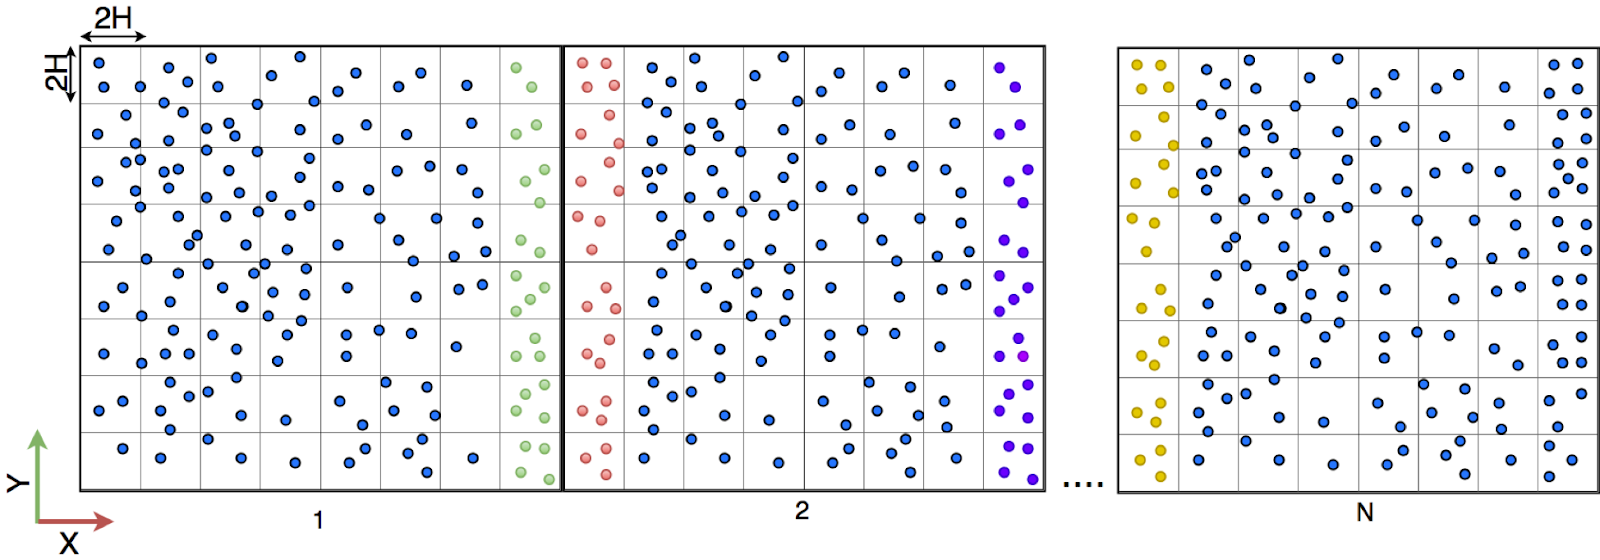
\includegraphics[scale=0.30]{distrib2}
  }
  \caption{Распределение данных между устройствами для алгоритма PCI SPH, разделение пространства показано красными вертикальными линиями, стрелкой с надписью G обозначено направление вектора гравитации.}
  \label{fig:dstr_2}
\end{figure}

% Нужно дополнить эту секцию
\fixme {На рисунке \ref{fig:dstr_3} показана схема выделения и использования памяти. Каждый экземпляр класса Solver управляет памятью на своем устройстве, при этом общий массив данных хранится оперативной памяти и управляется в хостовой части программы.}
\begin{figure}[ht]
  \centerfloat{
    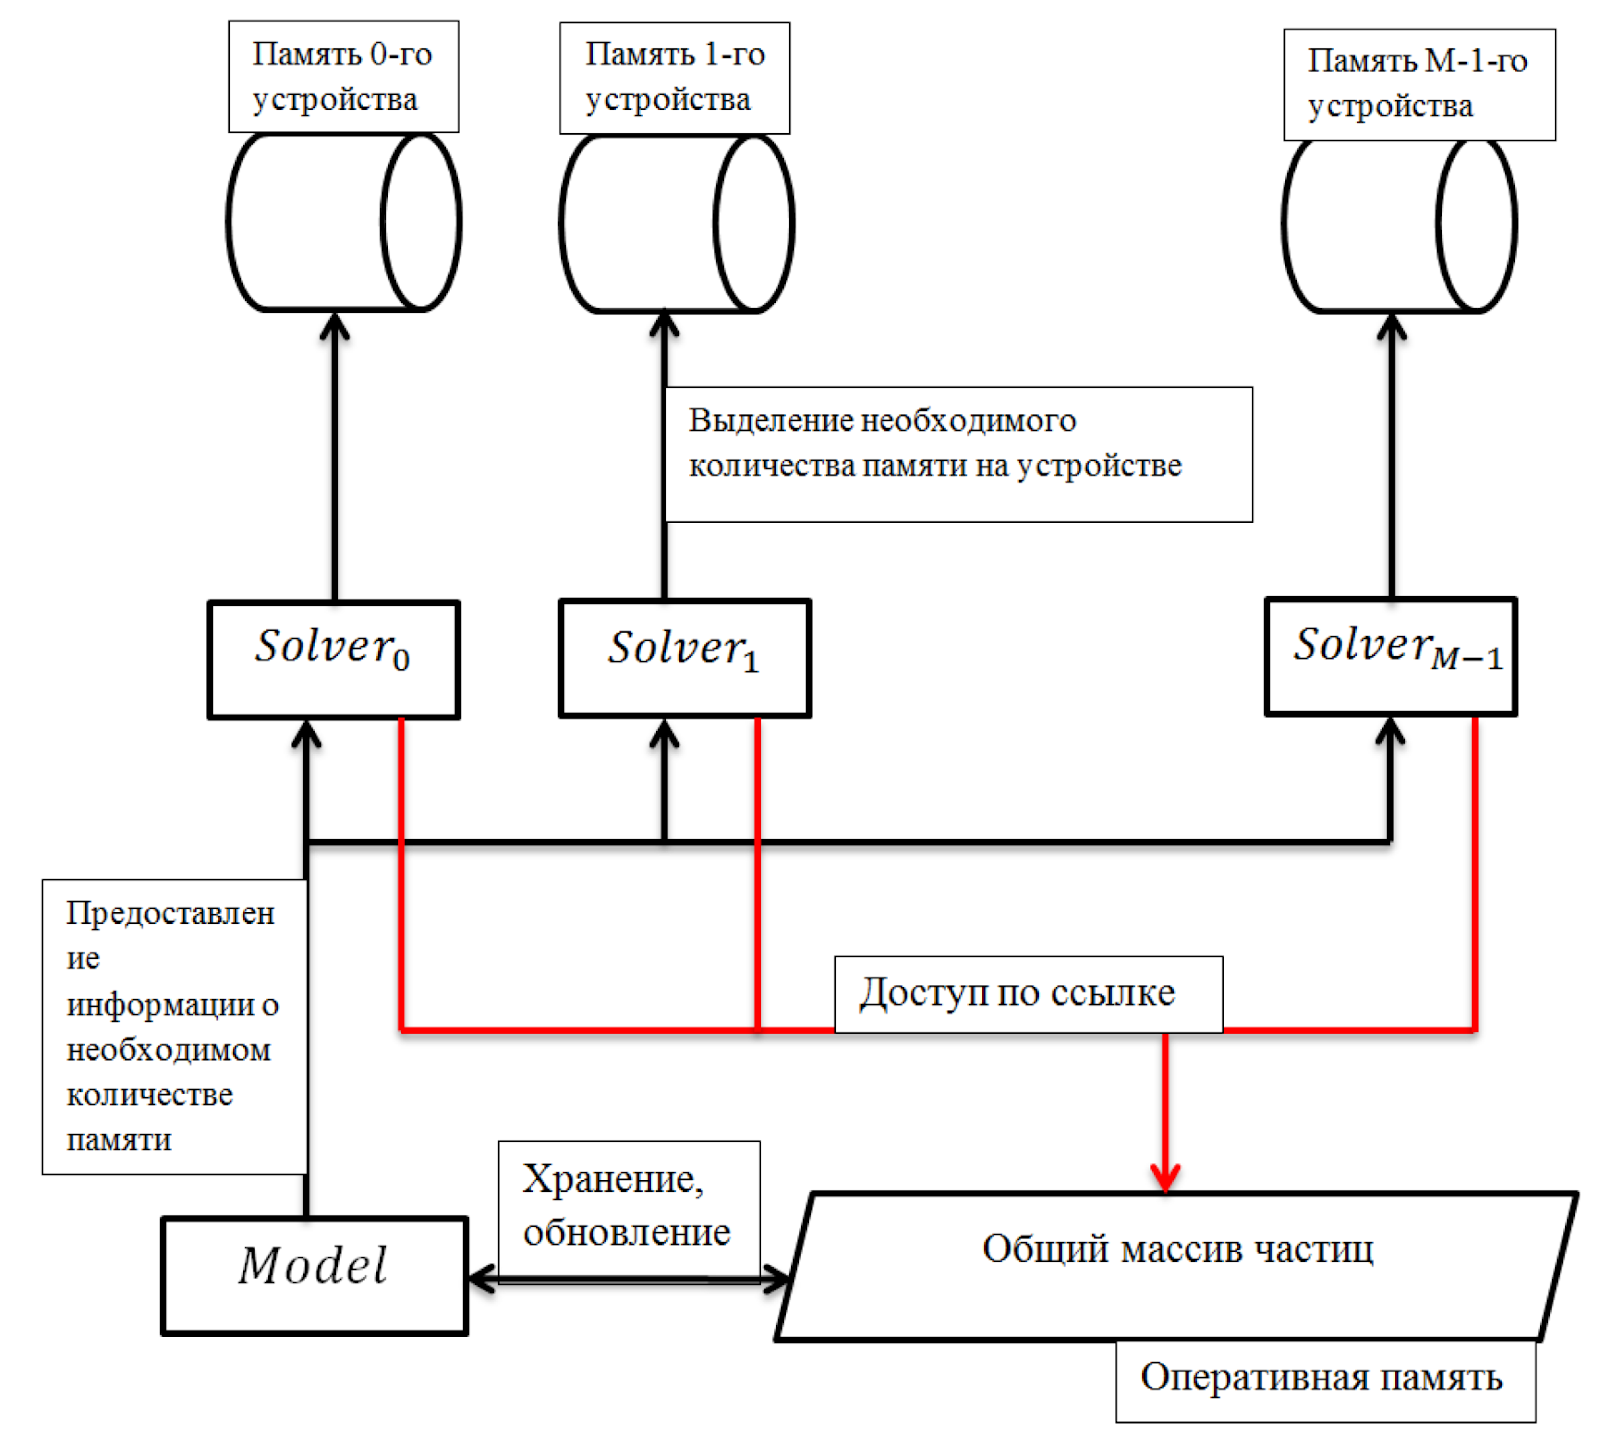
\includegraphics[scale=0.20]{distrib3}
  }
  \caption{Схема использования и выделения памяти.}
  \label{fig:dstr_3}
\end{figure}

